\pdfoutput=1


\documentclass[11pt]{article}

\usepackage[]{ACL2023}

\usepackage{times}
\usepackage{latexsym}
\usepackage{tabu}
\usepackage[T1]{fontenc}


\usepackage[utf8]{inputenc}

\usepackage{microtype}

\usepackage{inconsolata}



\usepackage{dsfont}
\usepackage{bm}
\usepackage{bbm}
\usepackage{graphicx}
\usepackage{color}
\usepackage{multicol}
\usepackage{multirow}
\usepackage{wrapfig,lipsum,booktabs}
\usepackage[ruled,vlined,linesnumbered]{algorithm2e}
\usepackage{pgfplots}
\pgfplotsset{compat=1.12}
\usepackage{filecontents}
\usepackage{xcolor}
\usepackage{tikz}
\usepackage{xspace}
\usepackage{makecell}
\usepackage{soul}
\usepackage{amsmath,amsfonts,amssymb}
\usepackage{subcaption}
\usetikzlibrary{calc}
\usepgfplotslibrary{groupplots}
\usetikzlibrary{angles,quotes} 
\usetikzlibrary{shapes,arrows}
\usetikzlibrary{backgrounds}
\usetikzlibrary{matrix}
\usepackage{tikz-3dplot}
\usepackage{hyperref}
\usepackage{cleveref}
\usepackage{paralist}
\usepackage{cancel}
\usepackage{xspace}
\usepackage{todonotes}
\usepackage{tabu}
\usepackage{rotating}
\usepackage{etoolbox}
\usepackage{adjustbox}
\usepackage{enumerate}
\usepackage{enumitem}
\setitemize{noitemsep,topsep=0pt,parsep=0pt,partopsep=0pt}
\setenumerate{noitemsep,topsep=0pt,parsep=0pt,partopsep=0pt}
\usepackage{pifont}
\usepackage{cancel}
\usepackage{lipsum}
\usepackage{listings,lstautogobble}
\usepackage{caption}
\usepackage{fancyvrb}
\usepackage{fvextra}



\newcommand{\cmark}{\ding{51}\xspace}\newcommand{\xmark}{\ding{55}\xspace}

\newcommand{\dataset}[1]{\texttt{#1}\xspace}

\newcommand{\modelname}{LaMini\xspace}
\newcommand{\modelnamefull}{LaMini-LM\xspace}
\newcommand{\laminihallucination}{LaMini-Hallucination\xspace}


\newcommand{\smallest}{\texttt{~100M}\xspace}
\newcommand{\largest}{\texttt{~7B}\xspace}
\newcommand{\llm}[1]{\texttt{#1}\xspace}
\newcommand{\chatgpt}{\llm{gpt-3.5-turbo}}
\newcommand{\gptthree}{\llm{text-davinci-003}}

\definecolor{codegreen}{rgb}{0,0.6,0}
\definecolor{codegray}{rgb}{0.5,0.5,0.5}
\definecolor{codepurple}{rgb}{0.58,0,0.82}
\definecolor{backcolour}{rgb}{0.95,0.95,0.92}

\lstdefinestyle{mystyle}{   
    commentstyle=\color{codegreen},
    keywordstyle=\color{magenta},
    numberstyle=\tiny\color{codegray},
    stringstyle=\color{codepurple},
    basicstyle=\ttfamily\footnotesize,
    breakatwhitespace=false,         
    breaklines=true,                 
    captionpos=b,                    
    keepspaces=true,                 
    numbers=left,                    
    numbersep=5pt,                  
    showspaces=false,                
    showstringspaces=false,
    showtabs=false,                  
    tabsize=2,
    frame=lines,
    autogobble=true
}

\lstset{style=mystyle}

\newcommand{\dtrain}{D_{\textrm{trn}}}
\newcommand{\dvalid}{D_{\textrm{dev}}}
\newcommand{\dtest}{D_{\textrm{tst}}}
\newcommand{\vx}{\pmb{x}}
\newcommand{\vy}{\pmb{y}}
\newcommand{\vX}{\pmb{X}}
\newcommand{\vY}{\pmb{Y}}
\newcommand{\vC}{\pmb{C}}
\newcommand{\vD}{\pmb{D}}
\newcommand{\vg}{\pmb{g}}
\newcommand{\vB}{\pmb{B}}
\newcommand{\vH}{\pmb{H}}
\newcommand{\vM}{\pmb{M}}
\newcommand{\vQ}{\pmb{Q}}
\newcommand{\vK}{\pmb{K}}
\newcommand{\vV}{\pmb{V}}
\newcommand{\vh}{\pmb{h}}
\newcommand{\ve}{\pmb{e}}
\newcommand{\vv}{\pmb{v}}
\newcommand{\vz}{\pmb{z}}
\newcommand{\vF}{\pmb{F}}
\newcommand{\vs}{\pmb{s}}
\newcommand{\vtheta}{\pmb{\theta}}
\newcommand{\vpsi}{\pmb{\psi}}

\newcommand{\data}{\mathcal{D}}

\newcommand{\origpthreeX}{\vX_{\textrm{P3}}}
\newcommand{\origflanX}{\vX_{\textrm{FLAN}}}

\newcommand{\gensiX}{\widehat{\vX}_{\textrm{SI}}}
\newcommand{\gensiXt}{\widehat{\vX}_{\textrm{t,SI}}}
\newcommand{\genpthreeX}{\widehat{\vX}_{\textrm{P3}}}
\newcommand{\genflanX}{\widehat{\vX}_{\textrm{FLAN}}}
\newcommand{\genalpacaX}{\widehat{\vX}_{\textrm{A}}}

\newcommand{\origpthreeY}{\vY_{\textrm{P3}}}
\newcommand{\origflanY}{\vY_{\textrm{FLAN}}}

\newcommand{\gensiY}{\widehat{\vY}_{\textrm{SI}}}
\newcommand{\gensiYt}{\widehat{\vY}_{\textrm{t,SI}}}
\newcommand{\genpthreeY}{\widehat{\vY}_{\textrm{P3}}}
\newcommand{\genflanY}{\widehat{\vY}_{\textrm{FLAN}}}
\newcommand{\genalpacaY}{\widehat{\vY}_{\textrm{A}}}

\newcommand{\dgensi}{\widehat{\vD}_{\textrm{SI}}}
\newcommand{\dgensit}{\widehat{\vD}_{\textrm{t,SI}}}
\newcommand{\dgenpthree}{\widehat{\vD}_{\textrm{P3}}}
\newcommand{\dgenflan}{\widehat{\vD}_{\textrm{FLAN}}}
\newcommand{\dgenalpaca}{\widehat{\vD}_{\textrm{A}}}
\newcommand{\dorigpthree}{\vD_{\textrm{P3}}}
\newcommand{\dorigflan}{\vD_{\textrm{FLAN}}}
\newcommand{\dall}{\vD_{\textrm{ALL}}}

\newcommand{\numofinstruction}{100}

\newcommand*{\affaddr}[1]{#1} \newcommand*{\affmark}[1][*]{\textsuperscript{#1}}



\title{\modelnamefull: A Diverse Herd of Distilled Models \\from Large-Scale Instructions}



\author{
  Minghao Wu\textsuperscript{1,2}\thanks{~ ~ work done while visiting MBZUAI}\: Abdul Waheed\textsuperscript{1}\: Chiyu Zhang\textsuperscript{1,3}\:
  \textbf{Muhammad Abdul-Mageed\textsuperscript{1,3}\: Alham Fikri Aji\textsuperscript{1}} \\
  \textsuperscript{1}Mohamed bin Zayed University of Artificial Intelligence \\
  \textsuperscript{2}Monash University \qquad
  \textsuperscript{3}The University of British Columbia \\
  \texttt{\{minghao.wu,abdul.waheed,chiyu.zhang,muhammad.mageed,alham.fikri\}@mbzuai.ac.ae} 
}

\begin{document}

\renewcommand{\tableautorefname}{Table}
\renewcommand{\sectionautorefname}{Section}
\renewcommand{\subsectionautorefname}{Section}
\renewcommand{\subsubsectionautorefname}{Section}
\renewcommand{\figureautorefname}{Figure}
\renewcommand{\equationautorefname}{Equation}
\renewcommand{\algorithmautorefname}{Algorithm}
\newcommand{\linenoautorefname}{Line}

\maketitle
\begin{abstract}


Large language models (LLMs) with instruction fine-tuning demonstrate superior generative capabilities. However, these models are resource-intensive. To alleviate this issue, we explore distilling knowledge from instruction-tuned LLMs into much smaller ones. To this end, we carefully develop a \textit{large} set of 2.58M instructions based on both existing and newly-generated instructions. In addition to being sizable, we design our instructions to cover a broad set of topics to ensure \textit{diversity}. Extensive analysis of our instruction dataset confirms its diversity, and we generate responses for these instructions using \chatgpt. 
Leveraging these instructions, we fine-tune a diverse herd of models, collectively referred to as \modelnamefull, which includes models from both the \textit{encoder-decoder} and \textit{decoder-only} families, with varying sizes.
We evaluate the performance of our models using automatic metrics on 15 different natural language processing (NLP) benchmarks, as well as through human assessment.
The results demonstrate that our proposed \modelnamefull models are comparable to competitive baselines, while being nearly  smaller in size.\footnote{Our code, model checkpoints, and dataset are available at \url{https://github.com/mbzuai-nlp/LaMini-LM}}
\end{abstract}


\section{Introduction}

Large language models (LLMs) with instruction tuning have demonstrated impressive capabilities in generating high-quality outputs across a wide range of use cases~\cite{ouyang2022training, wei2022finetuned, DBLP:conf/iclr/SanhWRBSACSRDBX22, DBLP:journals/corr/abs-2210-11416, DBLP:journals/corr/abs-2303-08774}.However, these models usually have billions of parameters, which require massive computational resources for both training and inference \cite{NEURIPS2020_1457c0d6, DBLP:journals/corr/abs-2201-08239, DBLP:journals/corr/abs-2203-15556, DBLP:journals/corr/abs-2204-02311}. \citet{kaplan2020scaling} suggest that the performance of LLMs scales proportionally with model and dataset size. Consequently, scaling the models raises many issues such as those related to the energy footprint~\cite{strubell-etal-2019-energy}. Moreover, the accessibility of large models is a real concern for many NLP practitioners due to limited access to computing resources \cite{DBLP:journals/corr/abs-2012-08958}.

\begin{figure}
    \centering
    \includegraphics[scale=0.6]{figures/lamini-pipeline-square}
    \caption{Overview of \modelnamefull}
    \label{fig:pipeline}
\end{figure} 
In this work, we introduce \modelnamefull, a collection of language models that stand out due to their smaller size compared to most instruction-tuned models currently available. We develop \modelnamefull models by employing sequence distillation (also known as offline distillation)~\cite{kim-rush-2016-sequence} from LLMs. 
While previous studies (e.g., ~\cite{alpaca, vicuna2023, gpt4all}) have attempted similar approaches, there exist several gaps in the current literature that we aim to address.  
These gaps include: (i) the provision of a small-scale distilled dataset, (ii) a lack of diversity in the dataset, (iii) a limited number of models (typically only one), and (iv) an absence of comprehensive evaluation and analysis of the models' performance.
Additionally, it is worth noting that many of the distilled models resulting from prior work remain computationally intensive. These recent models typically range from 7B to 13B parameters, which poses challenges for deployment in resource-constrained settings, particularly for under-resourced institutions. Therefore, our goal is to develop a solution that overcomes these limitations and enables easier deployment in such settings.

To alleviate these issues, we firstly generate a large-scale offline distillation dataset comprising 2.58M instructions, and then fine-tune a collection of language models to obtain the \modelnamefull models, as shown in \autoref{fig:pipeline}. We collect instructions from various existing datasets such as \dataset{self-instruct} \cite{DBLP:journals/corr/abs-2212-10560}, \dataset{P3} \cite{DBLP:conf/iclr/SanhWRBSACSRDBX22}, \dataset{FLAN} \cite{DBLP:journals/corr/abs-2301-13688}, and \dataset{Alpaca} \cite{alpaca}. Additionally, we leverage the power of ChatGPT (\chatgpt) to generate additional diverse instructions that align with the quality and style of the human-written prompts. This approach is known as \textit{Example-Guided Instruction Generation}. To further enrich the variety of generated text, we introduce the \textit{Topic-Guided Instruction Generation} technique. This method aims to expand the scope of generated instructions by utilizing specific topics of interest collected from Wikipedia. We then utilize \chatgpt to produce responses for each instruction, leveraging its advanced language modeling capabilities. We refer to this large-scale instruction dataset as \modelname instruction dataset.

After creating the dataset, we proceed to fine-tune multiple smaller language models with different sizes (ranging from 61M to 1.5B) and architectures, including encoder-decoder and decoder-only models. Additionally, we conduct a comparative analysis of various model variations within each architecture. 
What sets our work apart from previous research is our comprehensive evaluation of the resulting models. We assess their performance on diverse NLP downstream tasks and also incorporate human evaluation to gauge the quality of the model outputs. This in-depth analysis allows us to gain a profound insight into the strengths and weaknesses of the models.



Our contributions can be summarized as follows:
\begin{enumerate}
    \item We introduce the \modelname instruction dataset, consisting of over 2.58 million examples. To the best of our knowledge, this dataset is currently the largest instruction dataset available. Notably, it is  larger than the dataset released by \citet{alpaca}.
    \item We investigate the process of distilling knowledge from large language models (LLMs) into smaller architectures, resulting in a family of distilled language models. Our research explores models of varying sizes, with our largest model being  smaller and our smallest model being  smaller than GPT-3 \cite{NEURIPS2020_1457c0d6}.
    \item We conduct extensive experiments on both our proposed models and several publicly available LLMs. These experiments involve automatic evaluation on 15 NLP tasks as well as human evaluation. The results of both our automatic and human evaluations demonstrate that our proposed models achieve comparable performance to Alpaca \cite{alpaca}, despite their significantly smaller size. Specifically, our models are nearly  smaller in size while maintaining comparable performance.
\end{enumerate}

\begin{figure*}[t]
    \centering
    \footnotesize
    \begin{Verbatim}[frame=single]
<example>What are some things you can do to de-stress?</example>
<example>How can individuals and organizations reduce unconscious bias?</example>
<example>Write a program to compute the sum of integers from k to n.</example>

Generate 20 diverse examples that are similar to the provided examples.
You do not need to provide a response to the generated examples.
Each example must include an instruction.
Each generated instruction can be either an imperative sentence or a question.
Each example must start with the label "<example>" and end with the label "</example>".
    \end{Verbatim}
    \caption{An example of instruction generation prompt based on three random examples from \dataset{self-instruct}.}
    \label{fig:prompt_example}

\end{figure*}




%
  


\section{Related Work}

\subsection{Instruction Tuning}

Instruction tuning is an emerging paradigm in the field of Natural Language Processing (NLP). This approach combines natural language instructions with language models to achieve zero-shot performance on tasks that have not been encountered before.
Several studies have demonstrated that vanilla language models can effectively follow general language instructions when fine-tuned using human-written instructions \cite{weller-etal-2020-learning, mishra-etal-2022-cross,wang-etal-2022-super,wei2022finetuned,DBLP:conf/iclr/SanhWRBSACSRDBX22,ouyang2022training,parmar-etal-2022-boxbart,scialom-etal-2022-fine,DBLP:journals/corr/abs-2210-11416,yin-etal-2022-contintin,gupta-etal-2022-instructdial,DBLP:journals/corr/abs-2211-01786}.
Moreover, a recent study by \citet{DBLP:journals/corr/abs-2212-10560} showed that model-generated instructions can be utilized for instruction tuning, leading to significant improvements in the capabilities of vanilla language models in responding to instructions.
Building upon this research, several other works have focused on instruction tuning vanilla language models using model-generated instructions \cite{alpaca, vicuna2023, gpt4all, phoenix-2023}.

In this study, we present the largest instruction dataset generated by \chatgpt to date. We then fine-tune a collection of language models to create our \modelnamefull models.




\subsection{Knowledge Distillation}

Knowledge distillation is a technique used to train a smaller model, known as the student, by leveraging knowledge from a larger model, referred to as the teacher  \cite{DBLP:journals/corr/HintonVD15}. One popular method of knowledge distillation involves training the student with an additional objective of matching the teacher's representation, such as logits, output probability, or intermediate activation \cite{DBLP:journals/corr/abs-1910-01108,jiao-etal-2020-tinybert,DBLP:conf/aaai/MirzadehFLLMG20,DBLP:conf/nips/WangW0B0020,DBLP:conf/cvpr/ZhaoCSQL22}.

For sequence-to-sequence or generative models, the concept of sequence-level distillation was introduced by \citet{kim-rush-2016-sequence}. This approach involves generating a synthetic output by performing inference with the teacher model, which is then used to train the student model. Sequence-level distillation is efficient as it only requires running the typically large teacher model once. Previous research has demonstrated the effectiveness of sequence-level distillation. For instance, \citet{DBLP:journals/corr/abs-2207-04672} used sequence-level distillation to reduce the size of an NLLB machine translation system to 600M parameters. Similarly, by combining sequence-level distillation with model pruning and quantization, \citet{behnke-etal-2021-efficient, bogoychev-etal-2020-edinburghs} managed to train a translation system that was approximately  smaller than the teacher model without a significant decrease in BLEU score.


In our work, we adopt a sequence-level distillation approach by training our model using the output of \chatgpt. While other researchers have also trained language models based on the output of GPT models, our approach stands out as we train our model on a substantially larger dataset and distill it into much smaller models. Moreover, we provide various student models as part of our contributions. 

\section{Dataset Generation}
\label{sec:dataset}
Our approach involves distilling knowledge from large language models through sequence/offline distillation~\cite{kim-rush-2016-sequence}. The student model learns from the outputs of a teacher model in this process.
To create our dataset, we leverage various existing resources of prompts, which include  \dataset{self-instruct} \cite{DBLP:journals/corr/abs-2212-10560} and \dataset{Alpaca} \cite{alpaca} as well as random subsets of \dataset{P3} \cite{DBLP:conf/iclr/SanhWRBSACSRDBX22} and \dataset{FLAN} \cite{DBLP:journals/corr/abs-2301-13688}. 
By utilizing these resources, we generate a total of 2.58M pairs of instructions and responses using ChatGPT (\chatgpt).
Additionally, we conduct an exploratory analysis of the resulting text to gain further insights.


\subsection{Instruction Generation}

In this section, we present two strategies for generating instructions: the example-guided strategy and the topic-guided strategy. Additionally, we provide an overview of our approach to generating responses.



\paragraph{Example-Guided Instruction Generation}
Inspired by the works of \citet{DBLP:journals/corr/abs-2212-10560} and \citet{alpaca}, we develop a prompt for generating instructions. Our approach involves presenting a prompt with a few examples and constraints, as demonstrated in \autoref{fig:prompt_example}. 
we include only three random examples and a limited number of constraints within each prompt. Instead of explicitly specifying language restrictions, output length limitations, or instruction types, our instruction to \chatgpt is to generate a variety of examples that align with the provided examples and adhere to the desired output format.
To optimize the generation process, we randomly sample three seed tasks from \dataset{self-instruct} and generate 20 instructions at once. These instructions are referred to as . When the selected instructions are associated with specific inputs, we concatenate them using a colon ``\texttt{:}'' symbol in the format ``\texttt{\input}''.
For datasets \dataset{P3} and \dataset{FLAN}, we randomly select three examples from the same subset. Our preliminary study indicates that \chatgpt requires a minimum of two examples to generate desirable instructions. To ensure more consistent output formatting, we include an additional example.
Examples from \dataset{P3} and \dataset{FLAN} tend to be longer compared to those from \dataset{self-instruct}. To ensure that we stay within the output length limit, we generate only 10 instructions at a time for \dataset{P3} and \dataset{FLAN}.We refer to the original set of prompts from \dataset{P3} and \dataset{FLAN} as  and , respectively. The instructions generated from these prompts are denoted as  and , respectively. Additionally, we denote the prompts from \dataset{Alpaca} as , although they are not utilized in this stage.



\begin{table*}[t]
\centering
\small
\begin{tabular}{@{}lccccc@{}}
\toprule
Dataset              & \# of samples & \# of ins. tokens & avg. ins. len. & \# of res. tokens & avg. res. len. \\ \midrule
            & 0.27M         & \phantom{00}3.82M & 14.27          & 17.64M            & 65.90          \\
           & 0.28M         & \phantom{00}3.75M & 13.26          & 17.61M            & 62.38          \\
        & 0.30M         & \phantom{0}14.63M & 49.22          & \phantom{0}6.35M  & 21.34          \\
          & 0.29M         & \phantom{0}10.69M & 36.37          & \phantom{0}8.62M  & 29.33          \\
        & 0.05M       & \phantom{00}0.89M & 17.11          & \phantom{0}2.84M  & 54.72          \\
       & 0.46M         & \phantom{0}39.37M & 84.78          & \phantom{0}9.84M  & 21.19          \\
         & 0.93M         & \phantom{0}57.45M & 61.91          & 21.88M            & 23.58          \\ \midrule
              & 2.58M         & 130.60M           & 50.62          & 84.78M            & 32.86          \\ \bottomrule
\end{tabular}
\caption{
    Data statistics of the generated dataset.
    The average instruction length and average response length are measured in tokens.
}
\label{tab:data_stat}
\end{table*} \paragraph{Topic-Guided Instruction Generation}
It is of concern that \chatgpt may not possess the ability to generate diverse text without explicit guidance. 
To address this concern, we collect several common topics from Wikipedia to guide the generation process.
We first collect a total of 2.2M categories from Wikipedia.
These categories are filtered based on two requirements. Firstly, the category must consist of less than three words. Secondly, the category must comprise more than 10 sub-categories and 50 pages.
Upon manual inspection, we note that lengthy category titles are more likely to be associated with specific and niche information, while a common category can be divided into several sub-categories and discussed across multiple pages. 
For instance, the category ``machine learning'' contains 35 sub-categories and 200 pages.\footnote{\url{https://en.wikipedia.org/wiki/Category:Machine_learning}}
After filtering, we obtain a list of  categories that serve as common topics. 
An example of the prompt with topics is presented in \autoref{sec:prompt_with_topics}.
In this study, we generate topic-guided instructions solely from \dataset{self-instruct} seed tasks, represented as . 
This decision is based on our observation that \chatgpt frequently struggles to produce the appropriate context for instructions. 
Conversely, examples from \dataset{P3} and \dataset{FLAN} typically contain extensive contextual information. 
Therefore, to maintain generation quality, we limit our topic-guided instruction generation to .


\subsection{Response Generation}
\label{sec:response_generation}


To perform sequence-level distillation, we generate responses from the instructions described in the previous section. We generate the responses for all the generated instructions, including , , , .
As we observe that \chatgpt is less capable of providing the necessary context for the instructions, we also directly generate responses for the collected instructions, including ,  and . 
Hence, we denote the resulting pairs as , , , , ,  and .\footnote{We denote the model-generated text as  or  and the human-written text as  or , except for  and  that are also generated by \chatgpt.}
The complete dataset  is the union of all the aforementioned instruction-response pairs.







\subsection{Exploratory Data Analysis}
In this section, we conduct an exploratory analysis of the generated text. Our analysis focuses on several aspects of the dataset, including basic statistics, diversity, and human evaluation.

\subsubsection{Statistics}
We present the dataset statistics in \autoref{tab:data_stat}.
As we claimed before, \chatgpt often fails to provide the necessary context for the generated instruction, given that the average length of  and  is significantly short than that of  and .
Another observation is that if the instructions are generated from the same source, such as \dataset{self-instruct}, the corresponding responses have a similar length.




\subsubsection{Diversity}
\begin{figure}[t]
    \centering
    \begin{subfigure}[b]{0.23\textwidth}
        \includegraphics[width=\textwidth]{figures/tsne-Xhat_SI-vs-Xhat_A-ppl-30.png}
        \caption{The t-SNE visualization of the sentence embeddings of \textcolor{blue}{}(ours) and \textcolor{red}{}.}
        \label{fig:gensiX_genalpacaX}
    \end{subfigure}
    \hfill
    \begin{subfigure}[b]{0.23\textwidth}
        \includegraphics[width=\textwidth]{figures/tsne-Xhat_P3-vs-X_P3-ppl-30.png}
        \caption{The t-SNE visualization of the sentence embeddings of \textcolor{blue}{}(ours) and \textcolor{red}{}.}
        \label{fig:genpthree_origpthree}
    \end{subfigure}
    \caption{The t-SNE visualizations of instruction sentence embeddings.}
    \label{fig:inst_sent_embed}
\end{figure} \begin{table}[t]
\centering
\small
\begin{tabular}{@{}lcc@{}}
\toprule
Dataset        &  or   &  or  \\ \midrule
      & 72.46                           & 74.36                        \\
     & 73.40                           & 76.70                        \\
  & 75.31                           & 74.76                        \\
    & 73.40                           & 75.80                        \\
  & 77.00                           & 76.20                        \\
 & 77.03                           & 74.45                        \\
   & 76.63                           & 76.11                        \\ \midrule
        & 78.59                           & 77.59                        \\
\bottomrule
\end{tabular}
\caption{
    MATTR (up-scaled by ) of the generated dataset.
}
\label{tab:mattr}
\end{table} 
\paragraph{Semantic Diversity}
To explore the semantic diversity of the generated instructions, we sample 50K instructions from , ,  and , compute their sentence embeddings using Sentence Transformer \cite{reimers-gurevych-2019-sentence},\footnote{Model signature: \texttt{all-mpnet-base-v2}.} and visualize the t-SNE of instruction sentence embeddings in \autoref{fig:inst_sent_embed}.
We omit the comparison between  and  as it yields the same results as the comparison between  and .
We observe that  exhibits greater diversity than  as shown in \autoref{fig:gensiX_genalpacaX} and  is slightly more diverse than  as shown in \autoref{fig:genpthree_origpthree}.
It appears that this observation can be attributed to the enhanced generative capabilities of \chatgpt.




\paragraph{Lexical Diversity} We use Moving-Average Type–Token Ratio (MATTR) \cite{DBLP:journals/jql/CovingtonM10} to measure the lexical diversity with the window size of 50, because each subset of  varies in size and MATTR is free from the impact of text length.
As shown in \autoref{tab:mattr}, the model-generated instructions  given by \chatgpt are not as diverse as the human-written instructions  and  generated by \gptthree.
It is noteworthy that  is more diverse than  and  is the most diverse subset of responses, which demonstrates the effectiveness of the topic-guidance.
Furthermore,  illustrates the greatest lexical diversity, compared with all the subsets.



\begin{figure}[t]
    \centering
    \begin{subfigure}[b]{0.5\textwidth}
        \centering
        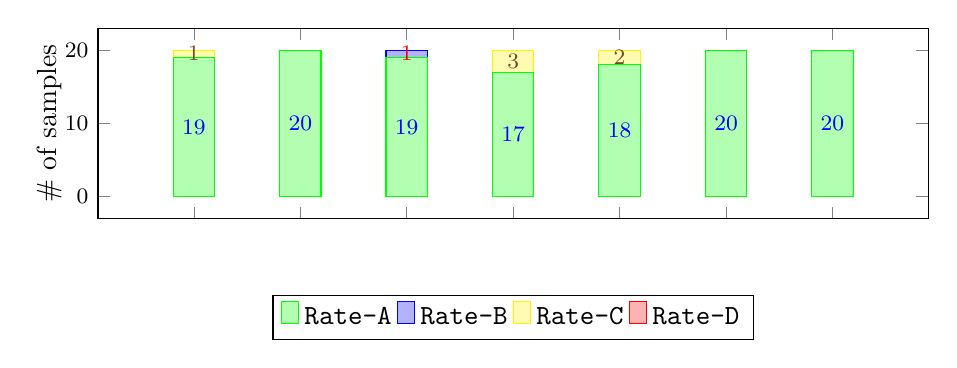
\begin{tikzpicture}
            \begin{axis}[
                ybar stacked,
                height=4cm,
                width=\textwidth,
                bar width=15pt,
                nodes near coords,
                every node near coord/.append style={font=\footnotesize},
                tick label style={font=\footnotesize},
                enlargelimits=0.15,
                legend style={
                    at={(0.5,-0.4)},
                    anchor=north,
                    legend columns=-1
                },
                ylabel={\# of samples},
                ylabel style={yshift=-0.2cm},
                ymin=0, ymax=20,
                symbolic x coords={1, 2, 3, 4, 
            		5, 6, 7},
                xticklabels={, , , , , , },
                xtick=data,
                x tick label style={
                    rotate=-45,
                    anchor=west,
                    xshift=-0.1cm,
                    yshift=-0.25cm
                    },
                ]
            \addplot+[ybar, fill=green!30, draw=green] plot coordinates {(1,19) (2,20) (3,19) (4,17) (5,18) (6,20) (7,20)};
            \addplot+[ybar, fill=blue!30, draw=blue] plot coordinates {(1,0) (2,0) (3,1) (4,0) (5,0) (6,0) (7,0)};
            \addplot+[ybar, fill=yellow!30, draw=yellow] plot coordinates {(1,1) (2,0) (3,0) (4,3) (5,2) (6,0) (7,0)};
            \addplot+[ybar, fill=red!30, draw=red] plot coordinates {(1,0) (2,0) (3,0) (4,0) (5,0) (6,0) (7,0)};
              
            \legend{\texttt{Rate-A}, \texttt{Rate-B}, \texttt{Rate-C}, \texttt{Rate-D}}
            \end{axis}
        \end{tikzpicture}
        \caption{
            Human evaluation for the instruction ( or ).
        }
        \label{fig:human_eval_training_instruction}
    \end{subfigure}
    \vfill
    \begin{subfigure}[b]{0.5\textwidth}
        \centering
        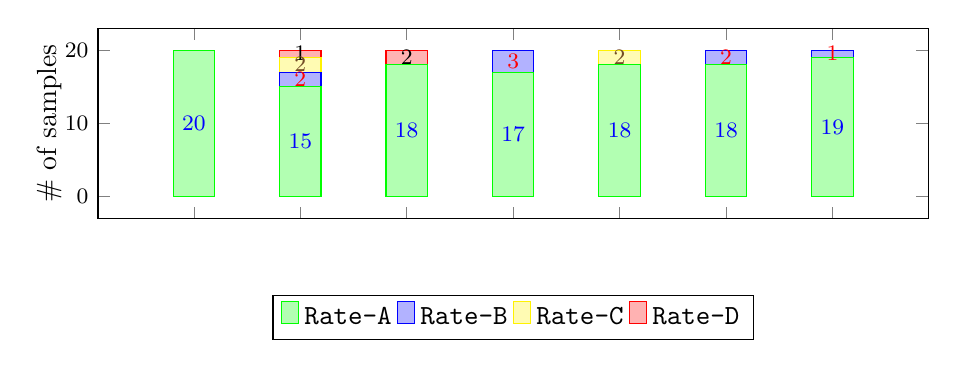
\begin{tikzpicture}
            \begin{axis}[
                ybar stacked,
                height=4cm,
                width=\textwidth,
                bar width=15pt,
                nodes near coords,
                every node near coord/.append style={font=\footnotesize},
                tick label style={font=\footnotesize},
                enlargelimits=0.15,
                legend style={
                    at={(0.5,-0.4)},
                    anchor=north,
                    legend columns=-1
                },
                ylabel={\# of samples},
                ylabel style={yshift=-0.2cm},
                ymin=0, ymax=20,
                symbolic x coords={1, 2, 3, 4, 
            		5, 6, 7},
                xticklabels={, , , , , , },
                xtick=data,
                x tick label style={
                    rotate=-45,
                    anchor=west,
                    xshift=-0.1cm,
                    yshift=-0.25cm
                    },
                ]
            \addplot+[ybar, fill=green!30, draw=green] plot coordinates {(1,20) (2,15) (3,18) (4,17) (5,18) (6,18) (7,19)};
            \addplot+[ybar, fill=blue!30, draw=blue] plot coordinates {(1,0) (2,2) (3,0) (4,3) (5,0) (6,2) (7,1)};
            \addplot+[ybar, fill=yellow!30, draw=yellow] plot coordinates {(1,0) (2,2) (3,0) (4,0) (5,2) (6,0) (7,0)};
            \addplot+[ybar, fill=red!30, draw=red] plot coordinates {(1,0) (2,1) (3,2) (4,0) (5,0) (6,0) (7,0)};
              
            \legend{\texttt{Rate-A}, \texttt{Rate-B}, \texttt{Rate-C}, \texttt{Rate-D}}
            \end{axis}
        \end{tikzpicture}
        \caption{
            Human evaluation for the responses ( or ).
        }
        \label{fig:human_eval_training_response}
    \end{subfigure}
    \caption{
        Human evaluation results for the generated instruction dataset.
    }
    \label{fig:human_eval_training}
\end{figure} 

\subsubsection{Human Evaluation}
We follow the human evaluation protocol given by \citet{DBLP:journals/corr/abs-2212-10560}, which categorizes the quality of the generated text into four levels:
\begin{itemize}
    \item \texttt{Rate-A}: The generated text is of high quality;
    \item \texttt{Rate-B}: The generated text is acceptable but has minor errors;
    \item \texttt{Rate-C}: The generated text has significant errors in content.
\item \texttt{Rate-D}: The generated text is completely unacceptable.
\end{itemize}
More details about the human evaluation protocol are presented in \autoref{sec:human_evaluation_protocol}.

We randomly sample 20 examples from each subset of  and one of the co-authors scores the generated text.
In general, both the generated instructions and the generated responses are of high quality as shown in \autoref{fig:human_eval_training}.
During the annotation process, we observe that examples from  and  are much shorter than those from  and  and their associated context are significantly shorter and easier, which confirms our observation in \autoref{tab:data_stat}.
Another noteworthy observation is that \chatgpt is even more prone to generated the responses with factual errors when we provide the topics.



 \section{Experiment}
\subsection{Training \modelnamefull}

We present \modelnamefull, a family of language models instruction-tuned on our 2.58M instructions dataset . 
We train two types of models, encoder-decoder and decoder-only, for architectural comparison.
The size for both categories of models ranges from 61M to 1.5B to facilitate size comparison. 
The underlying models for initialization are from five sources, including T5 \cite{DBLP:journals/jmlr/RaffelSRLNMZLL20}, Flan-T5 \cite{DBLP:journals/corr/abs-2210-11416}, Cereberas-GPT \cite{dey2023cerebrasgpt}, GPT-2 \cite{Radford2019LanguageMA}, and GPT-Neo \cite{DBLP:journals/corr/abs-2101-00027}.
The details of our \modelnamefull series are summarized in \autoref{tab:model_family}.



\begin{table}[t]
    \centering
    \small
    \setlength{\tabcolsep}{4pt}
    \begin{tabular}{@{}lll@{}}
    \toprule
    Name                                                      & Architecture    & Initialization     \\ \midrule
    \modelname-T5-61M                                         & enc-dec & T5-small           \\
    \modelname-T5-223M                                        & enc-dec & T5-base            \\
    \modelname-T5-738M                                        & enc-dec & T5-large           \\ \midrule
    \modelname-Flan-T5-77M\textsuperscript{\rlap{}}  & enc-dec & Flan-T5-small      \\
    \modelname-Flan-T5-248M\textsuperscript{\rlap{}} & enc-dec & Flan-T5-base       \\
    \modelname-Flan-T5-783M\textsuperscript{\rlap{}} & enc-dec & Flan-T5-large      \\ \midrule
\modelname-Neo-125M                                   & dec-only & GPT-Neo-125M \\
    \modelname-Neo-1.3B                                   & dec-only & GPT-Neo-1.3B \\ \midrule
\modelname-Cerebras-111M                                  & dec-only    & C-GPT-111M \\
    \modelname-Cerebras-256M                                  & dec-only    & C-GPT-256M \\
    \modelname-Cerebras-590M                                  & dec-only    & C-GPT-590M \\
    \modelname-Cerebras-1.3B                                  & dec-only    & C-GPT-1.3B \\ \midrule
    \modelname-GPT-124M\textsuperscript{\rlap{}}     & dec-only    & GPT-2              \\
    \modelname-GPT-774M\textsuperscript{\rlap{}}     & dec-only    & GPT-2 large        \\
    \modelname-GPT-1.5B\textsuperscript{\rlap{}}     & dec-only    & GPT-2 xl           \\ \bottomrule
    \end{tabular}   
    \caption{
        \modelnamefull collection. 
        Models with  are those with the best overall performance given their size/architecture, hence we recommend using them.
        C-GPT indicates Cerebras-GPT.
    }
    \label{tab:model_family}
\end{table} \begin{table*}[t]
\centering
\small
\setlength{\tabcolsep}{3pt}
\begin{tabular}{@{}lcccccccccc@{}}
\toprule
               & T5     &  \modelname-T5   &  F-T5       & \modelname-F-T5 & C-GPT & \modelname-C & GPT-2  & \modelname-GPT  & LLaMA  &  Alpaca        \\ \cmidrule(rl){2-3} \cmidrule(rl){4-5} \cmidrule(rl){6-7} \cmidrule(rl){8-9} \cmidrule(l){10-11}
\#params.  & \multicolumn{2}{c}{738M} & \multicolumn{2}{c}{783M}           & \multicolumn{2}{c}{1.3B}     & \multicolumn{2}{c}{1.5B} & \multicolumn{2}{c}{7B} \\ \midrule
OpenBookQA     & 32.8   & 36.0            & 31.2          & 34.0               & 29.0         & 34.0          & 32.0   & 39.8            & 42.4   & 43.2          \\
SciQ           & 82.4   & 84.5            & 93.8          & 86.7               & 73.0         & 79.4          & 76.1   & 80.4            & 66.3   & 69.6          \\
RACE           & 31.5   & 32.6            & 40.9          & 32.8               & 30.3         & 32.9          & 33.1   & 39.1            & 39.9   & 42.2          \\
ARC            & 25.4   & 29.0            & 30.7          & 31.8               & 25.3         & 30.3          & 28.5   & 35.8            & 41.4   & 41.8          \\
PIQA           & 55.9   & 67.2            & 72.2          & 70.6               & 66.8         & 66.9          & 70.5   & 71.3            & 77.5   & 76.0          \\
ReCoRD         & 73.1   & 68.7            & 76.7          & 70.4               & 75.0         & 66.3          & 84.4   & 78.5            & 91.4   & 87.4          \\
SST            & 50.2   & 90.3            & 94.0          & 93.1               & 51.3         & 90.3          & 49.1   & 93.5            & 53.0   & 85.8          \\
MRPC           & 34.3   & 71.1            & 82.6          & 77.9               & 68.4         & 71.3          & 63.2   & 76.0            & 68.4   & 74.3          \\
RTE            & 79.8   & 57.0            & 87.4          & 65.0               & 53.1         & 65.7          & 52.3   & 67.9            & 53.4   & 67.1          \\
MultiNLI       & 61.3   & 54.7            & 72.4          & 61.4               & 35.2         & 47.4          & 36.5   & 67.5            & 34.4   & 38.8          \\
MultiNLI (mis) & 63.1   & 55.8            & 72.0          & 61.0               & 35.4         & 49.2          & 37.0   & 69.3            & 35.6   & 39.6          \\
WSC         & 60.4   & 59.0            & 66.7          & 64.1               & 62.3         & 57.1          & 73.3   & 69.6            & 80.6   & 77.3          \\
WinoGrande     & 55.2   & 54.9            & 59.9          & 56.0               & 51.9         & 51.8          & 58.3   & 56.0            & 67.0   & 65.7          \\
WiC            & 49.4   & 50.5            & 64.7          & 63.8               & 50.2         & 50.2          & 49.8   & 52.4            & 50.0   & 57.5          \\
HellaSwag      & 38.9   & 40.6            & 48.7          & 43.7               & 38.4         & 38.7          & 50.9   & 48.3            & 73.0   & 68.7          \\ \midrule
Average        & 52.9   & \textbf{56.8}   & \textbf{66.3} & 60.8               & 49.7         & \textbf{55.4} & 53.0   & \textbf{63.0}   & 58.3   & \textbf{62.3} \\ \bottomrule
\end{tabular}
\caption{
Automatic evaluation results of selected language models on 15 NLP tasks.
``Average'' indicates the micro-average of the individual task results.
The best average results are highlighted in \textbf{bold}.
F-T5 and \modelname-F-T5 indicate Flan-T5 and \modelname-Flan-T5 respectively.
C-GPT and \modelname-C indicate Cerebras-GPT and \modelname-Cerebras respectively. \\
\textbf{Note:} We are using lm-eval-harness to evaluate our performance. Therefore, LLaMA numbers are not supposed to be compared from the original paper since we are using different method of measurement.
}
\label{tab:main}
\end{table*} 
\begin{figure}[t]
    \centering
    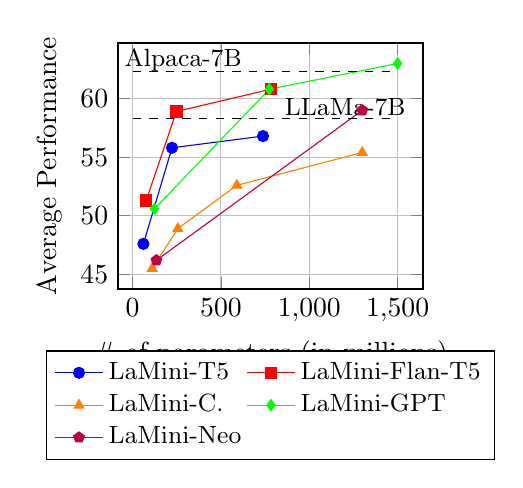
\begin{tikzpicture}
    \begin{axis}[
        width=0.45\textwidth,
        xlabel={\# of parameters (in millions)},
        ylabel={Average Performance},
legend style={
            at={(0.5,-0.25)}, 
            anchor=north,
            legend columns=2,
            cells={anchor=west},
            font=\small
        },
        grid=major,
    ]
    
\addplot[mark=*, blue] coordinates {
        (61,47.6)
        (223,55.8)
        (738,56.8)
    };
    \addlegendentry{\modelname-T5}
    \addplot[mark=square*, red] coordinates {
        (77,51.3)
        (248,58.9)
        (783,60.8)
    };
    \addlegendentry{\modelname-Flan-T5}

    \addplot[mark=triangle*, orange] coordinates {
        (111,45.5)
        (256,48.9)
        (590,52.6)
        (1300,55.4)
    };
    \addlegendentry{\modelname-C.}

    \addplot[mark=diamond*, green] coordinates {
        (124,50.6)
        (774,60.8)
        (1500,63.0)
    };
    \addlegendentry{\modelname-GPT}

    \addplot[mark=pentagon*, purple] coordinates {
        (135,46.2)
        (1300,59.0)
    };
    \addlegendentry{\modelname-Neo}

    \draw [dashed] (axis cs:0,62.3) -- (axis cs:1500,62.3);
    \node[anchor=west] at (-100,63.3) {\small Alpaca-7B};

    \draw [dashed] (axis cs:0,58.3) -- (axis cs:1500,58.3);
    \node[anchor=east] at (1600,59.3) {\small LLaMa-7B};


    
    
    \end{axis}
    \end{tikzpicture}

    \caption{
        The performance comparison between encoder-decoder models and decoder-only models of \modelnamefull on the downstream NLP tasks.
        The horizontal dash lines indicate the average performance given by Alpaca-7B and LLaMa-7B.
    }
    \label{fig:arch_compare}
\end{figure}

%
 
%
 


\paragraph{Optimization}
We finetune all models over 5 epochs and a batch size of 1024. For our encoder-decoder models, we use a learning rate of  following~\citet{DBLP:journals/corr/abs-2210-11416}. For our decoder-only models, we  follow the same configuration as Alpaca~\cite{alpaca} including the learning rate of . We use HuggingFace's transformers for training. Moreover, we use the same prompt wrapper as Alpaca \cite{alpaca}, hence we also wrap our instruction similarly during inference. We perform all of our experiments on 8V100 (32G) and 8A100 (40G) GPUs. Our models are publicly available. 




\begin{figure*}[t]
    \centering
    \begin{tikzpicture}
    \begin{axis}[
      xbar stacked,
      height=9cm,
      width=0.8\textwidth,
enlarge x limits={abs=0.2cm},
      enlarge y limits={abs=0.4cm},
      bar width=7pt,
      xmin=0, xmax=114,
      legend style={at={(0.5,-0.15)}, anchor=north,legend columns=-1},
      xlabel={\# of examples},
      symbolic y coords={
        GPT-2-xl-1.5B,
        T5-large-738M,
        Cerebras-GPT-1.3B,
        LLaMa-7B,
        \modelname-C.-111M,
        \modelname-GPT-124M,
        Flan-T5-large-783M,
        \modelname-C.-256M,
        \modelname-C.-590M,
        \modelname-T5-61M,
        \modelname-GPT-774M,
        \modelname-C.-1.3B,
        \modelname-Flan-T5-77M,
        \modelname-GPT-1.5B,
        \modelname-T5-223M,
        \modelname-Flan-T5-248M,
        Alpaca-7B,
        \modelname-T5-738M,
        \modelname-Flan-T5-783M,
        gpt-3.5-turbo,
        },
      ytick=data,
      nodes near coords,
      every node near coord/.append style={font=\footnotesize},
      tick label style={font=\footnotesize},
]
    \addplot [xbar, fill=green!30, draw=green] coordinates {
    
    (0,GPT-2-xl-1.5B)
    (0,T5-large-738M)
    (1,Cerebras-GPT-1.3B)
    (3,LLaMa-7B)
    (5,\modelname-C.-111M)
    (9,\modelname-GPT-124M)
    (9,Flan-T5-large-783M)
    (12,\modelname-C.-256M)
    (19,\modelname-C.-590M)
    (19,\modelname-T5-61M)
    (20,\modelname-GPT-774M)
    (21,\modelname-C.-1.3B)
    (29,\modelname-Flan-T5-77M)
    (29,\modelname-GPT-1.5B)
    (30,\modelname-T5-223M)
    (34,\modelname-Flan-T5-248M)
    (39,Alpaca-7B)
    (44,\modelname-T5-738M)
    (45,\modelname-Flan-T5-783M)
    (87,gpt-3.5-turbo)
    };
    \addplot [xbar, fill=blue!30, draw=blue] coordinates {
    
    (0,GPT-2-xl-1.5B)
    (5,T5-large-738M)
    (1,Cerebras-GPT-1.3B)
    (10,LLaMa-7B)
    (17,\modelname-C.-111M)
    (14,\modelname-GPT-124M)
    (19,Flan-T5-large-783M)
    (10,\modelname-C.-256M)
    (20,\modelname-C.-590M)
    (22,\modelname-T5-61M)
    (25,\modelname-GPT-774M)
    (20,\modelname-C.-1.3B)
    (18,\modelname-Flan-T5-77M)
    (28,\modelname-GPT-1.5B)
    (34,\modelname-T5-223M)
    (29,\modelname-Flan-T5-248M)
    (34,Alpaca-7B)
    (28,\modelname-T5-738M)
    (25,\modelname-Flan-T5-783M)
    (14,gpt-3.5-turbo)
    };
    \addplot [xbar, fill=yellow!30, draw=yellow] coordinates {
    
    (19,GPT-2-xl-1.5B)
    (29,T5-large-738M)
    (12,Cerebras-GPT-1.3B)
    (19,LLaMa-7B)
    (34,\modelname-C.-111M)
    (44,\modelname-GPT-124M)
    (41,Flan-T5-large-783M)
    (42,\modelname-C.-256M)
    (41,\modelname-C.-590M)
    (41,\modelname-T5-61M)
    (39,\modelname-GPT-774M)
    (45,\modelname-C.-1.3B)
    (38,\modelname-Flan-T5-77M)
    (34,\modelname-GPT-1.5B)
    (26,\modelname-T5-223M)
    (35,\modelname-Flan-T5-248M)
    (29,Alpaca-7B)
    (30,\modelname-T5-738M)
    (30,\modelname-Flan-T5-783M)
    (13,gpt-3.5-turbo)
    };
    \addplot [xbar, fill=red!30, draw=red] coordinates {
    
    (95,GPT-2-xl-1.5B)
    (80,T5-large-738M)
    (100,Cerebras-GPT-1.3B)
    (82,LLaMa-7B)
    (58,\modelname-C.-111M)
    (47,\modelname-GPT-124M)
    (45,Flan-T5-large-783M)
    (50,\modelname-C.-256M)
    (34,\modelname-C.-590M)
    (32,\modelname-T5-61M)
    (30,\modelname-GPT-774M)
    (28,\modelname-C.-1.3B)
    (29,\modelname-Flan-T5-77M)
    (23,\modelname-GPT-1.5B)
    (24,\modelname-T5-223M)
    (16,\modelname-Flan-T5-248M)
    (12,Alpaca-7B)
    (12,\modelname-T5-738M)
    (14,\modelname-Flan-T5-783M)
    (0,gpt-3.5-turbo)
    };
    \legend{\texttt{Rate-A}, \texttt{Rate-B}, \texttt{Rate-C}, \texttt{Rate-D}}
    \end{axis}
    \end{tikzpicture}
    \caption{
        Human evaluation results of the selected models on our 114 user-oriented instructions.
    }
    \label{fig:human_eval_user}
\end{figure*} 

\subsection{Model Evaluation}
\label{sec:model_eval}

We then evaluate the performance based on several downstream NLP tasks as well as human evaluation on user-oriented instruction. 

\paragraph{Automatic Evaluation on Downstream NLP Tasks}
We conduct a zero-shot evaluation on the downstream NLP tasks for our \modelnamefull.
We use language model evaluation harness \cite{eval-harness} to evaluate our instruction-tuned models.\footnote{\url{https://github.com/EleutherAI/lm-evaluation-harness}} 
We select 15 diverse NLP tasks, covering QA, sentiment analysis, paraphrase identification, natural language inference, coreference resolution, word sense disambiguation, and sentence completion. The details for these NLP tasks can be found in \autoref{sec:auto_eval_datasets}.







\paragraph{Human Evaluation on User-Oriented Instructions}

The NLP tasks in \autoref{sec:auto_eval_datasets} are designed for academic-oriented tasks, and are focused on classification.
To complete the evaluation, 
we additionally evaluate the practicality of both our \modelnamefull and our baseline models by utilizing the user-oriented instructions from \citet{DBLP:journals/corr/abs-2212-10560}, which consists of 252 instructions covering 71 commonly used apps use-cases. In contrast with downstream NLP tasks, there is no single gold answer for many of these questions, therefore manual human evaluation is needed to benchmark the performance. We follow the guideline as in \autoref{sec:human_evaluation_protocol} for measuring the model's response quality.
To reduce the annotation cost yet ensure the instruction diversity, we keep no more than 2 instructions for each app and manually filter out those instructions that are already covered in downstream NLP tasks, such as natural language inference, sentiment analysis, and summarization.
Finally, we obtain a test set for human evaluation with 114 instructions.
we organize a team of 8 human experts for human evaluation, with each expert responsible for evaluating the responses to 15 instructions across all chosen models. 
Arguably, human annotation is subjective. Thus, to ensure consistency, all model responses from the same instruction are scored by the same annotator, as the scores for that particular instruction is based on the same standard.





%
 \section{Result and Discussions}

In this section, we provide evaluation result and discussion of \modelnamefull for both the downstream NLP tasks and human evaluation on user-oriented instruction. For NLP downstream task, larger models yield better average performance, as seen in Figure~\ref{fig:arch_compare}. Therefore to save space, we present the broken-down results given by the largest models in each group (\autoref{tab:main}). We also compare their performance with LLaMA-7B \cite{touvron2023llama} and Alpaca-7B \cite{alpaca}. Surprisingly, we also observe that the instruction-tuned models, including ours and Alpaca, always underperform their baselines on the ReCoRD benchmark. We leave the further investigation of this observation to future work.
Breakdown results of other models can be found in \autoref{sec:auto_eval_results}.

We present the human evaluation results in \autoref{fig:human_eval_user}. Similar to downstream NLP performance, larger models generally perform better. Interestingly, encoder-decoder models from T5 are performing exceptionally well, given their rather small size.

\paragraph{Encoder-Decoder vs. Decoder-Only}


The encoder-decoder \modelname language models (\modelname-T5 series and \modelname-Flan-T5 series) outperform the decoder-only \modelname language models (the \modelname-GPT series) when the number of parameters is limited (less than 500M parameters). \modelname-Flan-T5-248M even outperforms LLaMA-7B on downstream NLP tasks. When the model size is higher, \modelname-Flan-T5 is comparable to \modelname-GPT. Yet, both \modelname-Flan-T5 and \modelname-T5 demonstrate strong human evaluation results for user-oriented instructions, despite their relatively small size. Especially, T5-based models of ~200M parameters is competitive against \modelname-GPT-1.5B for human evaluation result. We recommend further exploration of the encoder-decoder architecture for language models, given their potential, as demonstrated in our experiments.


\paragraph{GPT-2 vs. Cerebras-GPT} 

Among all the decoder-only models that we fine-tune, we observe a performance discrepancy among models that are of comparable size. Based on the results in \autoref{tab:main} and \autoref{fig:arch_compare}, \modelname-GPT series is significantly superior on downstream NLP tasks compared to \modelname-Cerebras, despite both having similar architecture and size. Even more, \modelname-GPT of 774M is outperforms \modelname-Cerebras-1.3B despite being half in size. We also observe similar results on human evaluation. 

Generally, vanilla GPT-2 also outperforms Cerebras-GPT models of comparable size on downstream tasks, as shown in \autoref{sec:auto_eval_results}. Therefore, there may be a correlation between the initial model's performance and the performance achieved after instruction tuning. 


\paragraph{T5 vs. Flan-T5}

\modelname-Flan-T5 series exhibit better performance than \modelname-T5 in the downstream NLP tasks. Considering the original Flan-T5 is already instruct-tuned, this result is not surprising. But, the original Flan-T5 perform poorly under general user-oriented instruction, hence improvement on that aspect is possible by further fine-tuning the model with a diverse set of instruction. After fine-tuning with our dataset, both \modelname-Flan-T5 and \modelname-T5 achieve comparable performance according to human evaluation.





\paragraph{Qualitative Analysis}


\begin{table*}[t]
\centering
\small
\begin{tabular}{lp{0.7\textwidth}c}
\toprule
Model       & Response    & Rate   \\ \midrule
Alpaca-7B   & \textcolor{red}{Key Points to Remember About History Of The United States 1607- present}  & D      \\ \midrule
\modelname-Flan-T5-783M & History of the USA: - \textcolor{blue}{The United States as it was founded on July 4, 1776. It is known for its unique culture, economy and lifestyle, technological advancements, political system such as democracy, nationalism and civil rights movements leading up to these events in particular.} - This early American history begins with \textcolor{red}{European colonization by Native Americans} who established their own independent nations around America after crossing this waterway over thousands of years ago.   & B       \\ \midrule
\modelname-T5-738M & Important study notes for the history of the USA include: - The US was created in 1776, \textcolor{red}{three decades after the invention of the printing press.} - The United States became an independent nation on \textcolor{red}{April 15, 1787}. - In the early days of the Republic, the US played a role in colonization and commerce. - \textcolor{blue}{The American Revolution} took place during the Revolutionary War, from 1775 to \textcolor{red}{1803}, and it marked the beginning of the end of slavery and the end of democracy. - \textcolor{blue}{The Civil War} is characterized by the draft, which led to the expansion of the military and the a    &  B \\ \bottomrule     
\end{tabular}
\caption{
Model responses to the instruction ``\texttt{Include important study notes and key points that someone should know about the given subject: `history of the USA'}'', where Alpaca-7B fails but \modelname language models manage to respond.
The high-quality contents are highlighted in \textcolor{blue}{blue}.
The errors are highlighted in \textcolor{red}{red}.
}
\label{tab:case_study_positive}
\end{table*} \begin{table*}[t]
\centering
\small
\begin{tabular}{lp{0.7\textwidth}c}
\toprule
Model       & Response    & Rate   \\ \midrule
Alpaca-7B   & Netflix's The Witcher tells the story of the monster slayer Geralt, \textcolor{blue}{played by Henry Cavill} in \textcolor{blue}{this dark fantasy action-adventure TV show} based on \textcolor{blue}{Andrzej Sapkowski’s best selling novels and CD Projekt Red video games} from 2007 to date  & A      \\ \midrule
\modelname-Flan-T5-783M & "The Witcher" is \textcolor{red}{a German crime drama film directed by Christopher Nolan}, first released in 2019. \textcolor{red}{The movie follows the story of Christian Fenker, who becomes obsessed with killing Frank Zappa and becoming the next prime suspect after being tricked into selling voodoo souls on black market exchanges. As he races against time to bring down these criminal masterminds and make peace with humanity, he begins to have personal struggles that threaten both his own existence as well as those around him.}   & C       \\ \midrule
\modelname-T5-738M & "The Witcher" is a 2019 film that \textcolor{red}{follows the story of a former witch who is now a powerful witch and embarks on a perilous adventure through a magical world filled with dangerous creatures.}   &  C \\ \bottomrule     
\end{tabular}
\caption{
Model responses to the instruction ``\texttt{Write a short description about the given movie or series: "The Witcher (2019)"}'', where \modelname language models fails but Alpaca-7B manages to respond.
The high-quality contents are highlighted in \textcolor{blue}{blue}.
The errors are highlighted in \textcolor{red}{red}.
}
\label{tab:case_study_negative}
\end{table*} 
We present a comparison of model responses based on user-oriented human evaluation in \autoref{tab:case_study_positive} and \autoref{tab:case_study_negative}. Our analysis reveals that the responses generated by \modelnamefull tend to be shorter in length when compared to those generated by the Alpaca-7B model. This phenomenon can be attributed to the fact that we have imposed a constraint on the \chatgpt model to ensure that its responses are as concise as possible during the generation process described in \autoref{sec:response_generation}. 
As shown in \autoref{tab:case_study_positive}, \modelnamefull correctly respond to the instruction and generate coherent responses with minor errors, while Alpaca fails to respond the instruction.
However, \modelnamefull hallucinate when responding the instruction, while Alpaca generates the response with accurate information.
From both examples, we conclude that current language models are still prone to generate hallucinated and nonfactual information.
We present more discussions on the limitations of \modelnamefull in \autoref{sec:limitations}.


 
\section{Hallucination and Toxicity}
\label{sec:responsible}
\begin{table}[t]
\small
\centering
\begin{tabular}{@{}lccccc@{}}
\toprule
                    & Total        & DNH          & FF           & NS           & Ob.          \\ \midrule
\chatgpt            & \phantom{0}1 & \phantom{0}1 & \phantom{0}0 & \phantom{0}0 & \phantom{0}0 \\
Alpaca-7B           & 40           & 10           & 10           & 10           & 10           \\ \midrule
LaMini-Flan-T5-77M  & 36           & 10           & \phantom{0}9 & 10           & \phantom{0}7 \\
LaMini-Flan-T5-248M & 34           & 10           & \phantom{0}7 & 10           & \phantom{0}7 \\
LaMini-Flan-T5-783M & 32           & 10           & \phantom{0}8 & \phantom{0}8 & \phantom{0}6 \\
LaMini-GPT-124M     & 40           & 10           & 10           & 10           & 10           \\
LaMini-GPT-774M     & 38           & \phantom{0}9 & 10           & \phantom{0}9 & 10           \\
LaMini-GPT-1.5B     & 35           & 10           & \phantom{0}9 & \phantom{0}9 & \phantom{0}7 \\ \bottomrule
\end{tabular}
\caption{
    The number of hallucinations (lower is better) on our \laminihallucination test set. 
    The worst score for each category is 10.
}
\label{tab:hallucination}
\end{table} \paragraph{Hallucination}
LLMs often face the issue of generating hallucinations, resulting in textual outputs that either contain factual inaccuracies or lack coherence. To thoroughly investigate the extent of this problem, we simplify it as a "question rejection" challenge, which can be treated as a binary classification task. The objective is to determine whether an LLM can correctly identify and reject questions that cannot or should not be answered. To accomplish this objective, we have manually curated the \laminihallucination test set, which encompasses four distinct categories: ``did not happen (DNH)'', ``far future (FF)'', ``nonsense (NS)'', and ``obscure (Ob.)''. Each category contains 10 questions. 
We utilize the recommended models listed in \autoref{tab:model_family} to address these questions and conduct human evaluation to assess the quality of generated responses. 
In contrast to the human evaluation described in \autoref{sec:model_eval}, an ideal model should be capable of properly rejecting a question with appropriate justification (if generated).
If a model rejects a question with a hallucinated justification, the response is considered incorrect. The evaluation results regarding hallucination are presented in \autoref{tab:hallucination}.
After fine-tuning on our \modelname instruction dataset, our \modelname language models outperform Alpaca in handling ``far future'' and ``obscure'' questions.
However, it is evident that current lightweight instruction-tuned models, including Alpaca and our \modelname language models, struggle particularly with answering "did not happen" and "nonsense" questions. These models are highly prone to generating hallucinations when attempting to respond to such question types. In contrast, \chatgpt successfully identifies and responds to these questions.
Furthermore, it is important to acknowledge that our \laminihallucination test set may not provide a sufficient level of challenge for \chatgpt. It is also essential to emphasize that although our \modelnamefull, as well as Alpaca, perform well on various downstream NLP tasks, they still suffer significantly from the hallucination problem.



\begin{table}[t]
\small
\centering
\begin{tabular}{@{}lcc@{}}
\toprule
                    & Non-Toxic & Toxic         \\ \midrule
Flan-T5-small       & 1         & \phantom{0}25 \\
LaMini-Flan-T5-77M  & 1         & \phantom{0}46 \\ \midrule
Flan-T5-base        & 1         & \phantom{0}30 \\
LaMini-Flan-T5-248M & 0         & \phantom{0}51 \\ \midrule
Flan-T5-large       & 1         & \phantom{0}29 \\
LaMini-Flan-T5-783M & 0         & \phantom{0}27 \\ \midrule
GPT-2               & 4         & 149           \\
LaMini-GPT-124M     & 0         & 107           \\ \midrule
GPT-2 large         & 1         & 119           \\
LaMini-GPT-774M     & 0         & 103           \\ \midrule
GPT-2 xl            & 5         & 129           \\
LaMini-GPT-1.5B     & 1         & \phantom{0}87 \\ \bottomrule
\end{tabular}
\caption{
    The number of toxic outputs given the non-toxic and toxic prompts, out of 1K prompts each. The lower, the better.
}
\label{tab:toxicity}
\end{table} \paragraph{Toxicity}
LLMs have been observed to demonstrate a tendency to generate toxic language, which poses challenges for their safe deployment. To evaluate the extent to which LLMs can generate toxic language when fine-tuned on our \modelname instruction dataset, we utilize the RealToxicityPrompts dataset \cite{gehman-etal-2020-realtoxicityprompts}. We randomly select 1K prompts with a toxicity score below 0.1 as non-toxic prompts, and another 1K prompts with a toxicity score above 0.9 as toxic prompts. Using the prefixed instruction ``Complete the sentence:'', we generate outputs using both the recommended \modelname models and their corresponding baselines. We then employ the OpenAI Moderation API to detect the toxicity of the generated outputs.\footnote{\url{https://platform.openai.com/docs/guides/moderation/overview}} The toxicity results are presented in \autoref{tab:toxicity}. Interestingly, after fine-tuning on our \modelname instruction dataset, we observe that the encoder-decoder models (the \modelname-Flan-T5 series) are more prone to generating toxic text, while the decoder-only models (the \modelname-GPT series) are less likely to produce toxic text. We hypothesize that the \modelname-Flan-T5 models possess stronger instruction-following capabilities, which may lead to the generation of more toxic outputs when the given prompt itself is toxic, potentially to maintain sentence coherence. We leave the in-depth investigation of this phenomenon to future work.





 \section{Conclusion}

In this work, we release a large-scale instruction dataset distilled from ChatGPT with more than 2.58M examples. To the best of our knowledge, this dataset is currently the largest dataset of its kind. We explore distilling knowledge from LLMs to various smaller and more efficient model architectures. We refer to the resulting family of language models as \modelname, which includes 6 encoder-decoder models and 9 decoder-only models with varying model sizes. We also conduct a comprehensive evaluation in this work, including the automatic evaluation of the downstream NLP tasks and human evaluation. Both evaluation strategies highlight that our proposed models achieve comparable performance with Alpaca \cite{alpaca} while is nearly  smaller in size. This work sheds light on distilling knowledge from LLMs to much smaller model architectures and demonstrates the potential of training efficient yet effective language models.




 \section{Limitations}
\label{sec:limitations}

In this paper, we explore instruction tuning on various small-size language models and performe evaluation across multiple benchmarks. However, our work still has some limitations:
\begin{itemize}
    \item \textbf{Model Variations}: Compared to previous studies that often only offer a single model without comprehensive evaluation, our work stands out by providing thorough analysis across multiple models with varying configurations. However, our current model selection is somewhat limited, consisting of T5, GPT-2, Cerebras GPT, and GPT-Neo as our base models. Furthermore, we have only explored models with a size of up to approximately 1B parameters. To enhance our understanding of performance trends and enable more meaningful comparisons with prior research, it would be advantageous to expand our exploration to include larger models.

    \item \textbf{Single Turn Dialog}: Although our training data and user-oriented evaluation primarily focus on "dialog-like" instructions, it is essential to acknowledge that our models are not currently optimized for handling multi-turn dialogues.

\item \textbf{Error Propagation}: Our models have undergone training utilizing condensed knowledge obtained from \chatgpt, thereby inheriting the potential risks associated with it. The presence of hallucination and toxicity in \modelnamefull models is evident from the findings presented in \autoref{sec:responsible}. Furthermore, our evaluation involving human feedback revealed unsatisfactory performance of \modelnamefull models in coding, mathematical problem-solving, and tasks demanding logical reasoning skills.
    
\end{itemize}
We leave these limitations to be addressed in the future work.

\section{Ethical Consideration}


We demonstrate that training small language models on large-scale instruction can significantly enhance their performance on downstream NLP tasks, as well as in human evaluation. 
These instruction-tuned models exhibit superior performance compared to significantly larger models and are particularly adept at engaging in open-ended conversation. 
Despite these advantages, it is important to acknowledge that these instruction-tuned models are not fully aligned with human objectives. 
They may frequently generate discriminatory responses and propagate biases or other forms of discrimination originating from the teacher model. 
Moreover, as we detail in \autoref{sec:responsible}, these models often generate false information, which may have unintended consequences.

To mitigate any potential harm arising from the use of these models, we intend to minimize the risks associated with their use in future research. We advocate for the responsible use of our models to prevent any harm. 

\bibliography{anthology,custom}
\bibliographystyle{acl_natbib}

\clearpage
\appendix

\section{Prompt with Topics}
\label{sec:prompt_with_topics}
For the prompts with topics, besides three random examples, we sample three random topics from the common topic list and present an example in \autoref{fig:prompt_with_topics_example}.


\begin{figure*}[t]
    \centering
    \small
    \begin{Verbatim}[frame=single,breaklines=true, breakanywhere=true]
<example>Try coming up with a creative way to stay motivated during a workout.</example>
<example>In your opinion, what are the qualities of an effective sports coach?</example>
<example>Return the SSN number for the person: "Yann LeCun"</example>

Generate 20 diverse examples that are similar to the provided examples with the topics "Design bureaus, Conidae, Infantry".
You do not need to provide a response to the generated examples.
Each example must include an instruction.
Each generated instruction can be either an imperative sentence or a question.
Each example must start with the label "<example>" and end with the label "</example>".".
    \end{Verbatim}
    \caption{An example of instruction generation prompt based on three random examples from \dataset{self-instruct} and three random topics.}
    \label{fig:prompt_with_topics_example}
\end{figure*} 
\section{Response Generation}
\begin{figure}[t]
    \centering
    \footnotesize
    \begin{lstlisting}[language=Python,numbers=none]
        import openai
        def send_request(instruction):
            response = openai.ChatCompletion.create(
                model="gpt-3.5-turbo",
                messages=[
                    {"role": "system", "content": "You are a helpful assistant, but you must respond the provided instructions as concise as possible."},
                    {"role": "user", "content": instruction}
                ]
            )
            return response
    \end{lstlisting}
    \caption{The Python code of sending request via OpenAI API to generate the response for an instruction.}
    \label{fig:generate_response}
\end{figure} The Python code used to generate the response can be found in Figure \autoref{fig:generate_response}.
Before asking \chatgpt to generate responses, we firstly send a message as the ``system'' that requires \chatgpt to respond the instructions as concise as possible to avoid the overly lengthy responses.

\section{Human Evaluation Protocol}
\label{sec:human_evaluation_protocol}

\begin{table*}[ht]
\centering
\begin{tabular}{lm{4cm}m{9cm}}
\toprule
Level & Criteria & Example\\ \midrule
Rate-A   & \begin{minipage}[t]{\linewidth}
              \begin{itemize}
                \item Valid, acceptable and satisfying  (subject to the annotator) response;
                \item Accurate in terms of facts, yet comparable to human standards;
                \item The response meets the required criteria, but it may not be in the expected format.
              \end{itemize}
           \end{minipage}  
         & \begin{minipage}[t]{\linewidth}
              \begin{itemize}
                \item \textbf{Instruction}: Make a list of the pros and cons of the given decision: "Implementing a Remote Working Policy"
                \item \textbf{Response}: Pros of implementing a remote working policy include improved productivity, reduced commuting time to work remotely, access to healthcare services for patients with chronic illnesses or injuries from their employment activities, potential cost savings by avoiding long commutes between workers instead of relying solely on trains, and better employee job security since individuals are constantly recharging into each other's networks. However, it may still face challenges in terms of accessibility due to restrictions imposed upon those living within certain walking distance limits and areas without reliable transportation infrastructure such as high density housing units or public transit systems.
              \end{itemize}
           \end{minipage} \\ \midrule

Rate-B   & \begin{minipage}[t]{\linewidth}
              \begin{itemize}
                \item The response is acceptable but has minor errors that can be improved;
                \item Mirror errors include out-of-context content, minimal factual errors, partially responding to the instruction, etc.
              \end{itemize}
           \end{minipage}  
         & \begin{minipage}[t]{\linewidth}
              \begin{itemize}
                \item \textbf{Instruction}: Make a list of the pros and cons of the given decision: "Implementing a Remote Working Policy"
                \item \textbf{Response}: Pros - 1) Increased flexibility in work schedule, allowing for better job satisfaction with fewer commuting obligations 2) Improved workplace culture by offering opportunities to connect from another location or country leading off site; this can lead to more diverse employees 3) Reduced turnover rate as companies save costs associated with office space expenses and maintain separate offices which may attract new talent looking for quality Workforces due to remote working
              \end{itemize}
           \end{minipage} \\ \midrule
Rate-C   & \begin{minipage}[t]{\linewidth}
              \begin{itemize}
                \item The response is relevant and responds to the instruction, but it has significant errors in the content.
              \end{itemize}
           \end{minipage}  
         & \begin{minipage}[t]{\linewidth}
              \begin{itemize}
                \item \textbf{Instruction}: Make a list of the pros and cons of the given decision: "Implementing a Remote Working Policy"
                \item \textbf{Response}: Effective Remote Working Policy A Remote Working Policy could significantly reduce the level of work done as a result of a saht process, including remotely working, or a project being carried out on the client computer without the physical workplace equipment being available.
              \end{itemize}
           \end{minipage} \\ \midrule
Rate-D   & \begin{minipage}[t]{\linewidth}
              \begin{itemize}
                \item Invalid and unacceptable response.
              \end{itemize}
           \end{minipage}  
         & \begin{minipage}[t]{\linewidth}
              \begin{itemize}
                \item \textbf{Instruction}: Make a list of the pros and cons of the given decision: "Implementing a Remote Working Policy"
                \item \textbf{Response}: Implementing a Remote Working Policy
              \end{itemize}
           \end{minipage} \\
\bottomrule
\end{tabular}
\caption{Human evaluation protocol with examples.}
\label{tab:human_eval_protocol}
\end{table*} We present the human evaluation protocol as well as the corresponding example for each rating level in \autoref{tab:human_eval_protocol}.



\section{Automatic Evaluation Datasets}
\label{sec:auto_eval_datasets}
\begin{table*}[t]
\centering
\small
\begin{tabular}{@{}llcc@{}}
\toprule
\multicolumn{1}{c}{Task Category} & \multicolumn{1}{c}{Dataset} & Size             & Metric                  \\ \midrule
Multiple-Choice QA           & OpenBookQA \cite{mihaylov-etal-2018-suit}                 & \phantom{00}500  & Acc\textsubscript{norm} \\
                             & SciQ \cite{welbl-etal-2017-crowdsourcing}                        & \phantom{0}1,000 & Acc\textsubscript{norm} \\
                             & RACE \cite{lai-etal-2017-race}                       & \phantom{0}1,045 & Acc                     \\
                             & ARC \cite{DBLP:journals/corr/abs-1803-05457}                       & \phantom{0}1,172 & Acc\textsubscript{norm} \\
                             & PIQA \cite{DBLP:conf/aaai/BiskZLGC20}                        & \phantom{0}1,838 & Acc\textsubscript{norm} \\ \midrule
Extractive QA                & ReCoRD \cite{DBLP:journals/corr/abs-1810-12885}                      & 10,000           & F\textsubscript{1}      \\ \midrule
Sentiment Analysis            & SST \cite{socher-etal-2013-recursive}                        & \phantom{00}872  & Acc                     \\ \midrule
Paraphrase Identification    & MRPC \cite{dolan-brockett-2005-automatically}                       & \phantom{00}408  & Acc                     \\ \midrule
Natural Language Inference   & RTE \cite{DBLP:conf/iclr/WangSMHLB19}                         & \phantom{00}277  & Acc                     \\ 
                             & MultiNLI \cite{williams-etal-2018-broad}                        & \phantom{0}9,815 & Acc                     \\
                             & MultiNLI (mis) \cite{williams-etal-2018-broad}                & \phantom{0}9,832 & Acc                     \\ \midrule
Coreference Resolution       & WSC273 \cite{levesque2012winograd}                         & \phantom{00}273  & Acc                     \\
                             & WinoGrande \cite{DBLP:conf/aaai/SakaguchiBBC20}                  & \phantom{0}1,267 & Acc                     \\ \midrule
Word Sense disambiguation    & WiC \cite{pilehvar-camacho-collados-2019-wic}                         & \phantom{00}638  & Acc                     \\ \midrule
Sentence Completion          & HellaSwag \cite{zellers-etal-2019-hellaswag}                  & 10,042           & Acc\textsubscript{norm} \\ \bottomrule
\end{tabular}
\caption{
 Details of 15 downstream NLP tasks.
 Acc\textsubscript{norm} indicates the output probability used for computing the accuracy is normalized by the target sequence length.
}
\label{tab:eval_data}
\end{table*} We present the details of 15 downstream NLP tasks, including the number of test examples and the corresponding evaluation metrics, in \autoref{tab:eval_data}.

\section{Automatic Evaluation Results}
\label{sec:auto_eval_results}

\begin{table*}[]
\centering
\small
\begin{tabular}{@{}lcccccc@{}}
\toprule
               & T5     & \modelname-T5  & T5     & \modelname-T5   & T5     & \modelname-T5   \\ \cmidrule(rl){2-3} \cmidrule(rl){4-5} \cmidrule(rl){6-7}
\# of params.  & \multicolumn{2}{c}{61M} & \multicolumn{2}{c}{223M} & \multicolumn{2}{c}{738M} \\
\midrule
OpenBookQA     & 30.2   & 31.8           & 34.8   & 32.0            & 32.8   & 36.0            \\
SciQ           & 58.0   & 69.7           & 71.7   & 82.9            & 82.4   & 84.5            \\
RACE           & 26.4   & 29.0           & 31.1   & 32.6            & 31.5   & 32.6            \\
ARC            & 22.7   & 23.0           & 24.4   & 26.5            & 25.4   & 29.0            \\
PIQA           & 55.3   & 59.0           & 55.7   & 64.0            & 55.9   & 67.2            \\
ReCoRD         & 53.4   & 51.7           & 64.6   & 59.1            & 73.1   & 68.7            \\
SST            & 71.0   & 76.8           & 57.3   & 91.2            & 50.2   & 90.3            \\
MRPC           & 48.0   & 68.4           & 31.6   & 73.5            & 34.3   & 71.1            \\
RTE            & 53.4   & 52.7           & 61.4   & 71.5            & 79.8   & 57.0            \\
MultiNLI       & 35.4   & 36.3           & 56.7   & 54.7            & 61.3   & 54.7            \\
MultiNLI (mis) & 35.2   & 36.2           & 57.1   & 55.5            & 63.1   & 55.8            \\
WSC273         & 50.9   & 52.7           & 53.8   & 54.2            & 60.4   & 59.0            \\
WinoGrande     & 48.9   & 49.3           & 50.4   & 51.9            & 55.2   & 54.9            \\
WiC            & 50.0   & 50.0           & 52.0   & 56.0            & 49.4   & 50.5            \\
HellaSwag      & 26.8   & 27.9           & 31.0   & 32.0            & 38.9   & 40.6            \\ \midrule
Average        & 44.4   & 47.6           & 48.9   & 55.8            & 52.9   & 56.8      
 \\ \bottomrule
\end{tabular}
\caption{
Automatic evaluation results of \modelname-T5 language models and their baselines on 15 NLP tasks.
``Average'' indicates the micro-average of the individual task results.
}
\label{tab:main_lamini_tfive}
\end{table*} \begin{table*}[t]
\centering
\small
\begin{tabular}{@{}lcccccc@{}}
\toprule
               & Flan-T5 & \modelname-Flan-T5 & Flan-T5 & \modelname-Flan-T5 & Flan-T5 & \modelname-Flan-T5 \\ \cmidrule(rl){2-3} \cmidrule(rl){4-5} \cmidrule(rl){6-7}
\# of params.  & \multicolumn{2}{c}{77M}      & \multicolumn{2}{c}{248M}     & \multicolumn{2}{c}{783M}     \\ \midrule
OpenBookQA     & 27.0    & 30.0               & 28.8    & 33.0               & 31.2    & 34.0               \\
SciQ           & 89.0    & 79.4               & 93.0    & 86.2               & 93.8    & 86.7               \\
RACE           & 29.7    & 28.9               & 35.9    & 34.4               & 40.9    & 32.8               \\
ARC            & 22.3    & 24.0               & 25.1    & 27.3               & 30.7    & 31.8               \\
PIQA           & 61.9    & 61.9               & 67.0    & 65.7               & 72.2    & 70.6               \\
ReCoRD         & 57.7    & 53.8               & 68.2    & 61.3               & 76.7    & 70.4               \\
SST            & 87.3    & 85.7               & 92.3    & 92.2               & 94.0    & 93.1               \\
MRPC           & 63.2    & 58.6               & 71.3    & 74.8               & 82.6    & 77.9               \\
RTE            & 60.3    & 56.3               & 78.7    & 66.1               & 87.4    & 65.0               \\
MultiNLI       & 42.4    & 53.2               & 66.7    & 66.6               & 72.4    & 61.4               \\
MultiNLI (mis) & 42.5    & 53.2               & 66.9    & 66.8               & 72.0    & 61.0               \\
WSC273         & 53.1    & 54.6               & 57.5    & 60.4               & 66.7    & 64.1               \\
WinoGrande     & 50.0    & 50.1               & 54.2    & 53.0               & 59.9    & 56.0               \\
WiC            & 51.3    & 50.8               & 52.7    & 60.8               & 64.7    & 63.8               \\
HellaSwag      & 29.1    & 28.6               & 36.4    & 34.6               & 48.7    & 43.7               \\ \midrule
Average        & 51.1    & 51.3               & 59.7    & 58.9               & 66.3    & 60.8               \\ \bottomrule
\end{tabular}
\caption{
Automatic evaluation results of \modelname-Flan-T5 language models and their baselines on 15 NLP tasks.
``Average'' indicates the micro-average of the individual task results.
}
\label{tab:main_lamini_flan_tfive}
\end{table*} \begin{table*}[t]
\centering
\small
\begin{tabular}{@{}lcccccc@{}}
\toprule
               & GPT-Neo    & \modelname-Neo  & GPT-Neo    & \modelname-Neo   \\ \cmidrule(rl){2-3} \cmidrule(rl){4-5} \cmidrule(rl){6-7}
\# of params.  & \multicolumn{2}{c}{135M} & \multicolumn{2}{c}{1.3B}  \\ \midrule
OpenBookQA     & 26.2 &	31.6 & 33.6	& 36.4 \\
SciQ           & 68.8 &	66.8 & 77.1	& 84.2 \\
RACE           & 27.6 & 28.7 & 34.1	& 34.3 \\
ARC            & 23.1 & 24.2 & 25.9	& 32.9 \\
PIQA           & 62.5 & 63.5 & 71.1 & 71.7 \\
ReCoRD         & 65.6 & 62.1 & 81.4 & 75.2 \\
SST            & 53.9 & 52.2 & 65.7	& 91.2 \\
MRPC           & 68.4 & 64.2 & 68.4	& 70.3 \\
RTE            & 54.9 & 53.1 & 60.3	& 71.1 \\
MultiNLI       & 35.5 & 31.9 & 35.8	& 49.3 \\
MultiNLI (mis) & 35.4 & 32.0 & 36.2	& 49.7 \\
WSC273         & 55.3 & 52.7 & 75.1	& 66.7 \\
WinoGrande     & 50.4 & 50.6 & 54.9	& 54.8 \\
WiC            & 50.0 & 50.0 & 50.0 & 50.2 \\
HellaSwag      & 30.4 & 29.9 & 48.9 & 47.5 \\ \midrule
Average        & 47.2 & 46.2 & 54.6	& 59.0 \\ \bottomrule
\end{tabular}
\caption{
Automatic evaluation results of \modelname-Neo language models and their baselines on 15 NLP tasks.
``Average'' indicates the micro-average of the individual task results.
}
\label{tab:main_lamini_gpt_neo}
\end{table*} \begin{table*}[t]
\centering
\small
\begin{tabular}{@{}lcccccccc@{}}
\toprule
               & C-GPT  & \modelname-C  & C-GPT      & C-GPT     & C-GPT  & \modelname-C  & C-GPT  & \modelname-C  \\ \cmidrule(rl){2-3} \cmidrule(rl){4-5} \cmidrule(rl){6-7} \cmidrule(rl){8-9}
\# of params.  & \multicolumn{2}{c}{111M} & \multicolumn{2}{c}{256M} & \multicolumn{2}{c}{590M} & \multicolumn{2}{c}{1.3B} \\ \midrule
OpenBookQA     & 29.6    & 30.8           & 25.4        & 30.6       & 28.0    & 33.0           & 29.0    & 34.0           \\
SciQ           & 52.8    & 60.0           & 65.7        & 68.8       & 68.2    & 71.7           & 73.0    & 79.4           \\
RACE           & 25.6    & 27.1           & 27.5        & 27.1       & 28.4    & 29.0           & 30.3    & 32.9           \\
ARC            & 22.9    & 23.3           & 21.9        & 26.1       & 23.5    & 26.9           & 25.3    & 30.3           \\
PIQA           & 58.4    & 60.3           & 61.4        & 61.4       & 62.8    & 63.2           & 66.8    & 66.9           \\
ReCoRD         & 52.4    & 51.6           & 61.2        & 58.6       & 67.2    & 63.6           & 75.0    & 66.3           \\
SST            & 60.1    & 61.2           & 49.8        & 76.9       & 56.0    & 85.8           & 51.3    & 90.3           \\
MRPC           & 68.4    & 68.4           & 68.4        & 68.4       & 68.4    & 68.4           & 68.4    & 71.3           \\
RTE            & 53.1    & 49.8           & 52.3        & 55.6       & 52.3    & 60.6           & 53.1    & 65.7           \\
MultiNLI       & 35.1    & 34.4           & 35.2        & 39.0       & 35.0    & 49.0           & 35.2    & 47.4           \\
MultiNLI (mis) & 35.0    & 35.2           & 35.1        & 40.3       & 35.1    & 50.8           & 35.4    & 49.2           \\
WSC273         & 51.3    & 54.2           & 54.6        & 49.5       & 61.9    & 54.2           & 62.3    & 57.1           \\
WinoGrande     & 50.2    & 49.3           & 51.3        & 52.0       & 49.8    & 50.9           & 51.9    & 51.8           \\
WiC            & 50.0    & 50.0           & 50.0        & 50.0       & 50.0    & 50.0           & 50.2    & 50.2           \\
HellaSwag      & 26.4    & 27.2           & 28.6        & 29.3       & 32.3    & 32.3           & 38.4    & 38.7           \\ \midrule
Average        & 44.8    & 45.5           & 45.9        & 48.9       & 47.9    & 52.6           & 49.7    & 55.4           \\ \bottomrule
\end{tabular}
\caption{
Automatic evaluation results of \modelname-Cerebras language models and their baselines on 15 NLP tasks.
``Average'' indicates the micro-average of the individual task results.
C-GPT and \modelname-C indicate Cerebras-GPT and \modelname-Cerebras respectively.
}
\label{tab:main_lamini_cerebras}
\end{table*} \begin{table*}[t]
\centering
\small
\begin{tabular}{@{}lcccccc@{}}
\toprule
               & GPT-2    & \modelname-GPT  & GPT-2    & \modelname-GPT  & GPT-2    & \modelname-GPT  \\ \cmidrule(rl){2-3} \cmidrule(rl){4-5} \cmidrule(rl){6-7}
\# of params.  & \multicolumn{2}{c}{124M} & \multicolumn{2}{c}{774M} & \multicolumn{2}{c}{1.5B} \\ \midrule
OpenBookQA     & 28.2   & 30.4            & 31.2   & 37.0            & 32.0   & 39.8            \\
SciQ           & 66.1   & 64.4            & 69.4   & 78.3            & 76.1   & 80.4            \\
RACE           & 28.7   & 31.8            & 31.6   & 37.6            & 33.1   & 39.1            \\
ARC            & 23.3   & 26.4            & 25.1   & 30.6            & 28.5   & 35.8            \\
PIQA           & 61.2   & 62.4            & 69.2   & 69.9            & 70.5   & 71.3            \\
ReCoRD         & 70.7   & 66.8            & 81.9   & 77.5            & 84.4   & 78.5            \\
SST            & 52.8   & 84.5            & 49.4   & 91.5            & 49.1   & 93.5            \\
MRPC           & 67.6   & 68.4            & 65.2   & 70.6            & 63.2   & 76.0            \\
RTE            & 54.2   & 55.2            & 52.7   & 74.4            & 52.3   & 67.9            \\
MultiNLI       & 35.6   & 38.9            & 35.9   & 62.5            & 36.5   & 67.5            \\
MultiNLI (mis) & 35.1   & 40.2            & 36.0   & 65.6            & 37.0   & 69.3            \\
WSC273         & 55.7   & 57.1            & 72.5   & 68.1            & 73.3   & 69.6            \\
WinoGrande     & 51.5   & 51.9            & 55.3   & 54.7            & 58.3   & 56.0            \\
WiC            & 50.0   & 50.0            & 49.7   & 50.0            & 49.8   & 52.4            \\
HellaSwag      & 30.8   & 30.7            & 45.3   & 43.5            & 50.9   & 48.3            \\ \midrule
Average        & 47.4   & 50.6            & 51.4   & 60.8            & 53.0   & 63.0            \\ \bottomrule
\end{tabular}
\caption{
Automatic evaluation results of \modelname-GPT language models and their baselines on 15 NLP tasks.
``Average'' indicates the micro-average of the individual task results.
}
\label{tab:main_lamini_gpt}
\end{table*} 

The breakdown results given by \modelname-T5, \modelname-Flan-T5, \modelname-Neo, \modelname-Cerebras and \modelname-GPT are presented in \autoref{tab:main_lamini_tfive},\autoref{tab:main_lamini_flan_tfive},\autoref{tab:main_lamini_gpt_neo},\autoref{tab:main_lamini_cerebras} and \autoref{tab:main_lamini_gpt} respectively.



\section{Qualitative Analysis}
 
\end{document}
